\section{Software architecture}

\begin{definition}
    The \emph{architecture} of a software system defines the system in terms of computational components and the interactions among these components.

    In the context of a software system, the \emph{software architecture} represents the set of structures necessary to reason about the system. 
    These structures include software elements, their relationships, and properties associated with both.
\end{definition}
There are three fundamental structures relevant to software architecture:
\begin{itemize}
    \item Component-and-connector structures: these structures describe how the system is organized as a set of elements with runtime behavior (components) and their interactions (connectors). 
        They allow us to study runtime properties, such as availability and performance, as well as how these structures collaborate.
        \begin{figure}[H]
            \centering
            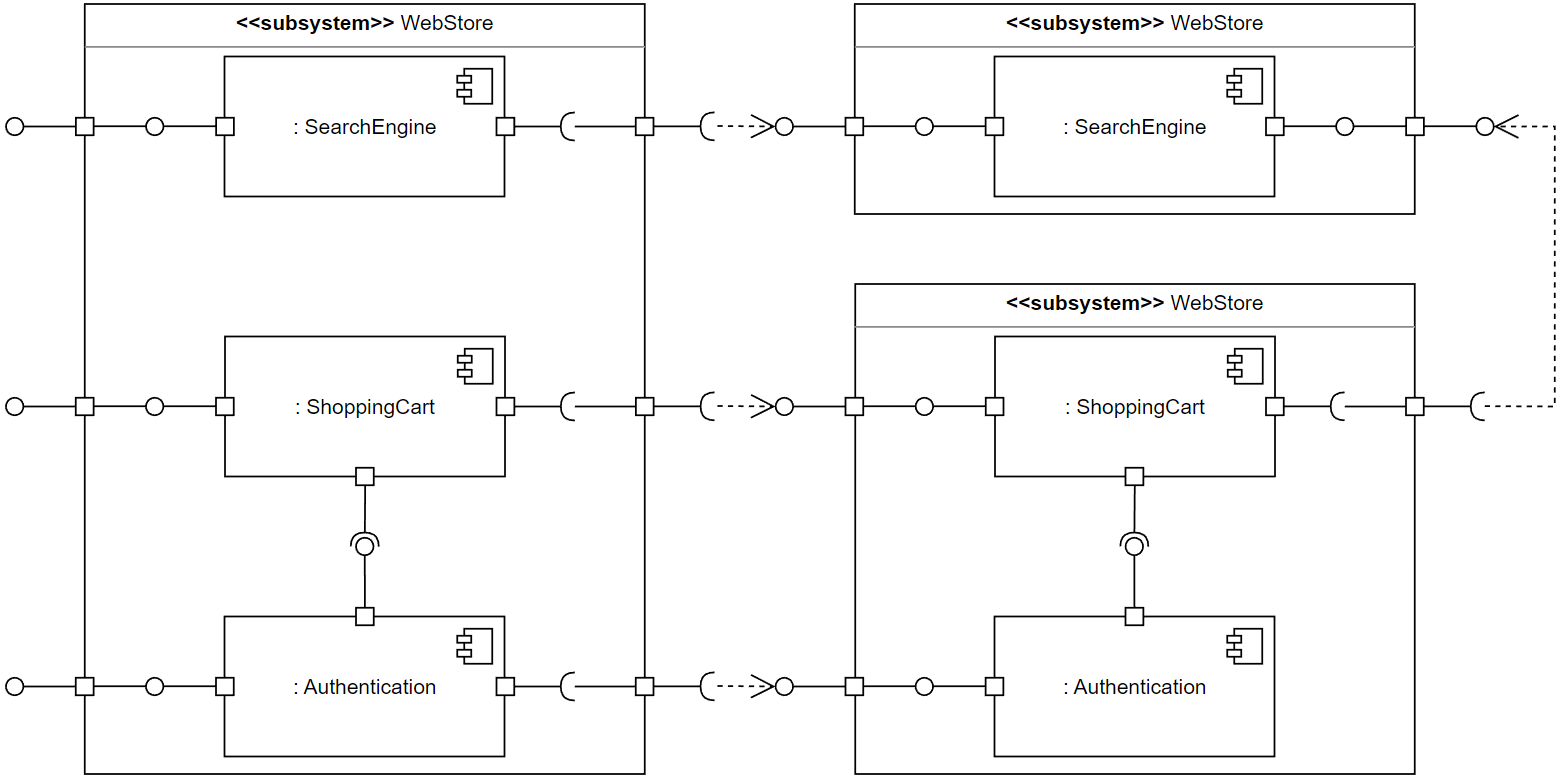
\includegraphics[width=0.75\linewidth]{images/component1.png}
            \caption{UML component diagrams for component and connector structure}
        \end{figure}
        \begin{figure}[H]
            \centering
            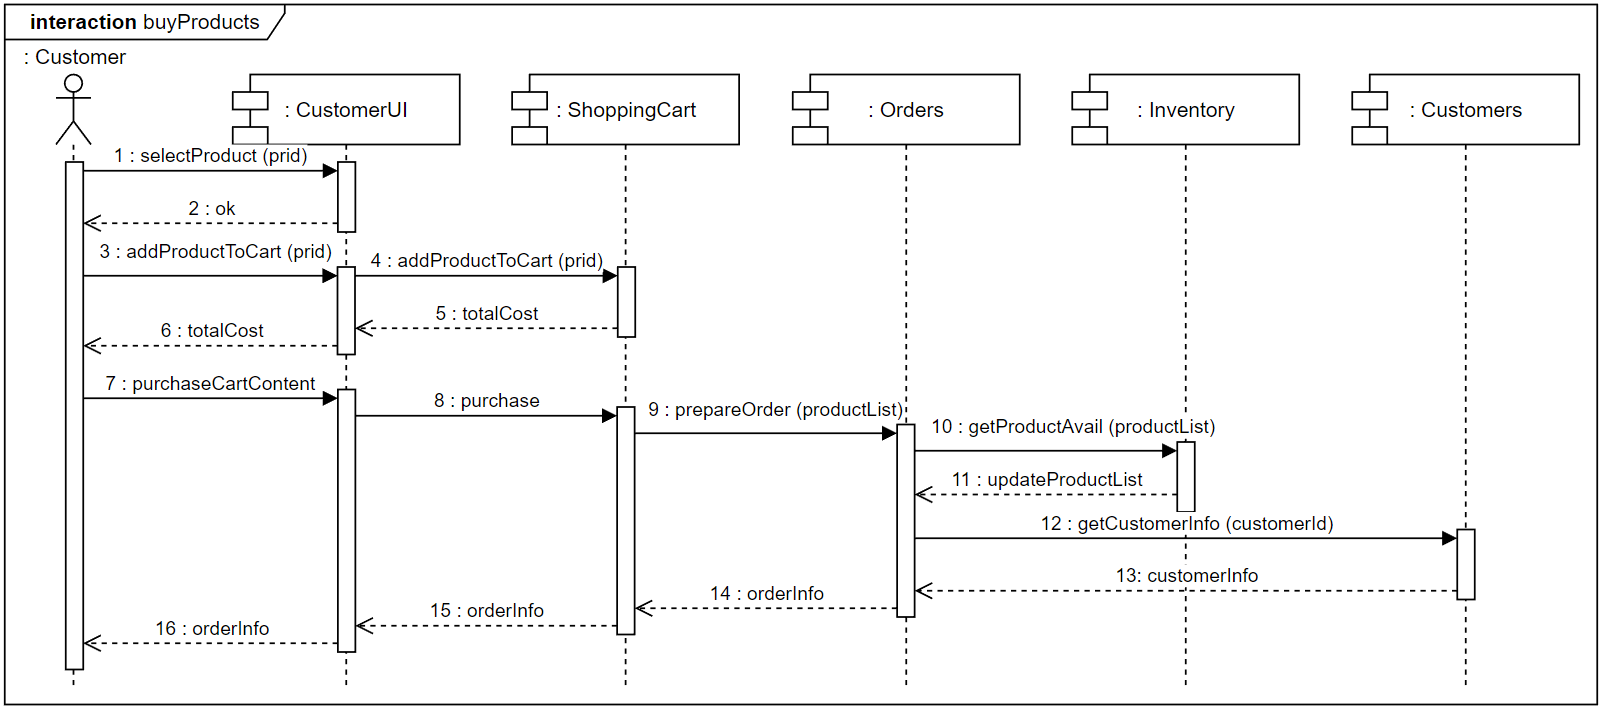
\includegraphics[width=0.75\linewidth]{images/component2.png}
            \caption{UML sequence diagrams for component and connector structure}
        \end{figure}
    \item Module structures: illustrate how a system is structured as a set of code or data units that need to be procured or constructed, along with their relationships. 
        Modules serve as implementation units and form the basis for work division.
        Typical relationships among these modules include "uses," "is-a" (generalization), and "is-part-of."
        \begin{figure}[H]
            \centering
            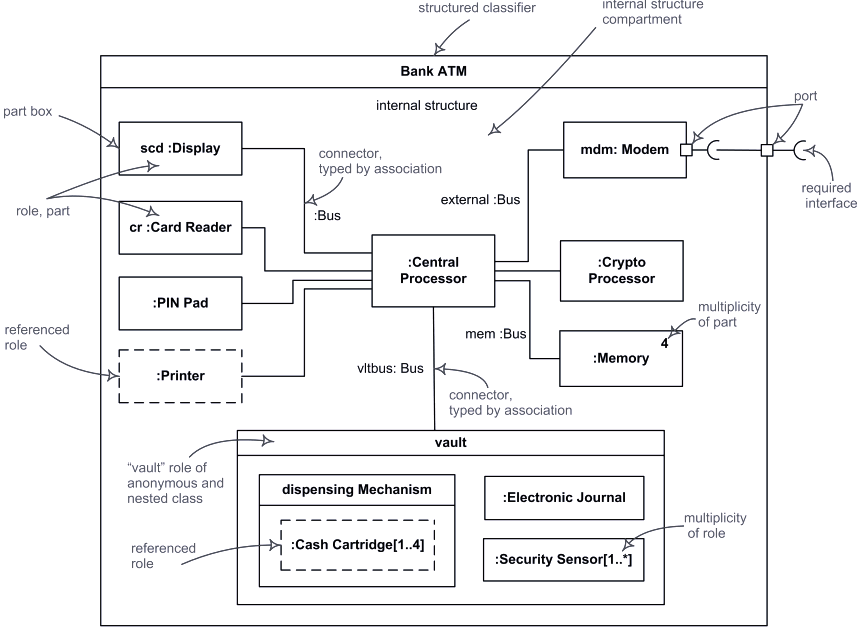
\includegraphics[width=0.75\linewidth]{images/modular1.png}
            \caption{UML composite structure diagram for module structure}
        \end{figure}
        \begin{figure}[H]
            \centering
            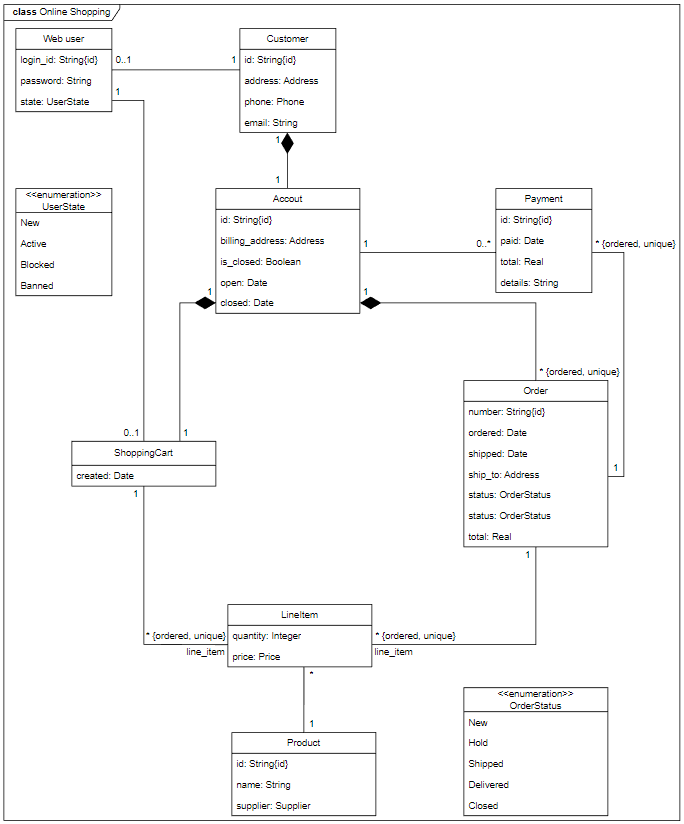
\includegraphics[width=0.7\linewidth]{images/modular2.png}
            \caption{UML class diagram for module structure}
        \end{figure}
        \begin{figure}[H]
            \centering
            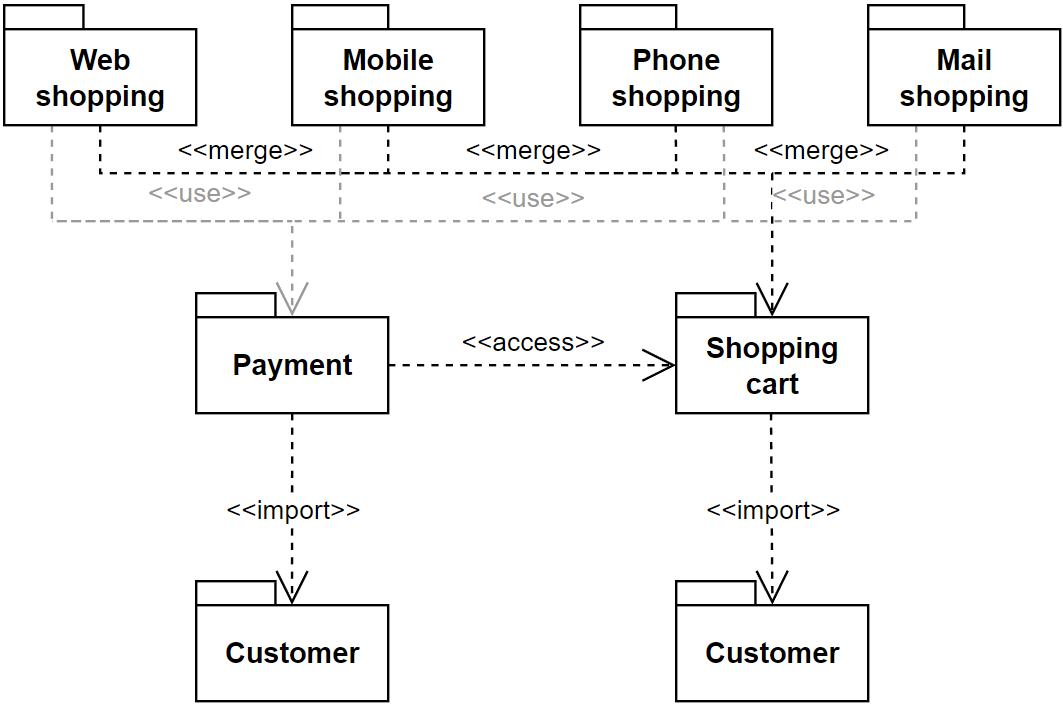
\includegraphics[width=0.7\linewidth]{images/modular3.png}
            \caption{UML package diagram for module structure}
        \end{figure}
    \item Allocation structures: these structures define how the elements from component and connector or module structures map to entities that are not software. 
        Common allocation structures include deployment structure, implementation structure, and work assignment structure. 
        The deployment structure captures the system's hardware topology, specifying the distribution of components and identifying performance bottlenecks.
        \begin{figure}[H]
            \centering
            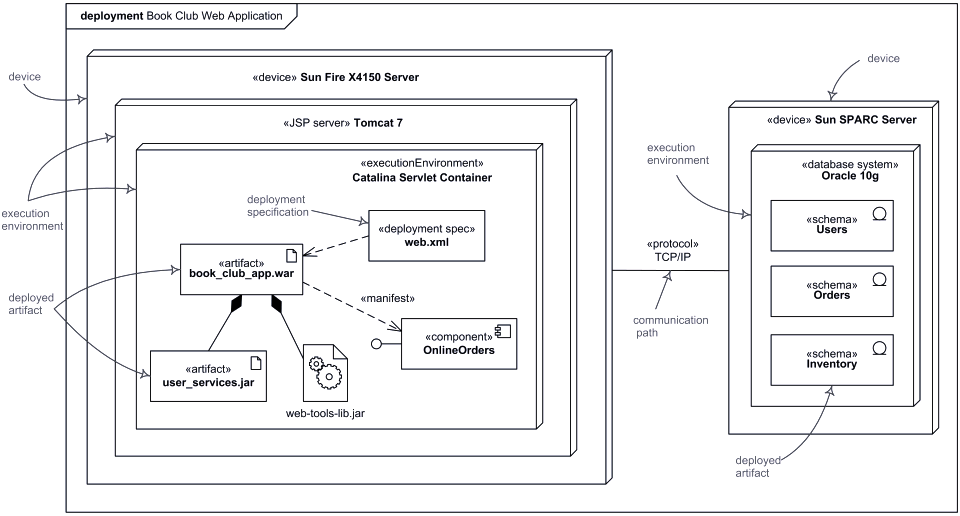
\includegraphics[width=1\columnwidth]{images/allocation1.png}
            \caption{UML deployment diagrams and deployment structure}
        \end{figure}
        \begin{figure}[H]
            \centering
            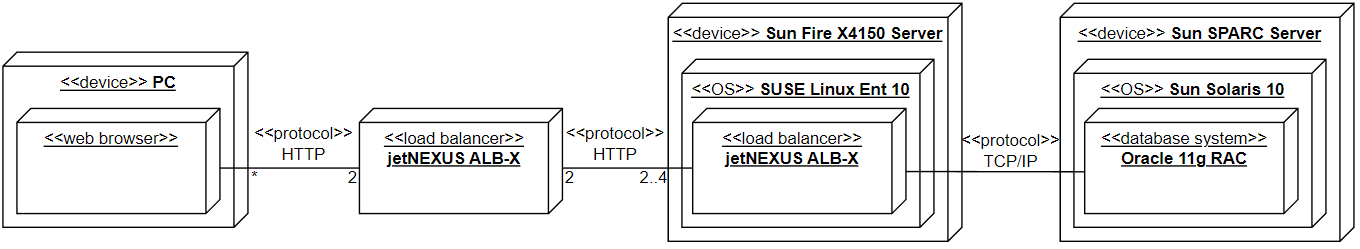
\includegraphics[width=1\columnwidth]{images/allocation2.png}
            \caption{UML deployment diagrams and deployment structure}
        \end{figure}
\end{itemize}

\subsection*{Summary}
\begin{table}[H]
    \centering
    \begin{tabular}{|c|ccc|}
    \hline
    \textbf{Structures}    & \textbf{Elements}                              & \textbf{Relations}                                                    & \textbf{Useful for}                                                                           \\ \hline
    Component diagrams     & \makecell{Components\\offering services}       & \makecell{Provided and\\required interfaces}                          & \makecell{Performance analysis\\Robustness analysis\\Resource allocation\\Project planning}   \\ \hline
    Sequence diagrams      & \makecell{Processes\\Threads}                  & \makecell{Synchronous and\\asynchronous\\messages}                     & \makecell{Analysis of\\resource contention\\Parallelism opportunities}                         \\ \hline
    \end{tabular}
    \caption{Component and connectors diagrams and usage}
\end{table}
\begin{table}[H]
    \centering
    \begin{tabular}{|c|ccc|}
    \hline
    \textbf{Structures}                                     & \textbf{Elements}                 & \textbf{Relations}                                                    & \textbf{Useful for}                                                               \\ \hline
    \makecell{Composite structures \\ Package diagrams}     & \makecell{Modules\\Packages}      & \makecell{Is a submodule of\\Uses}                                    & \makecell{Resource allocation\\Project planning\\Encapsulation}                   \\ \hline
    Class diagrams                                          & Classes                           & \makecell{Is-a\\Is part of}                                           & \makecell{Object-oriented development\\Planning for extensions}                   \\ \hline
    Layered structures                                      & -                                 & \makecell{Can use\\Provides abstraction}                              & Incremental development                                                           \\ \hline
    Data model                                              & Data entities                     & \makecell{One-to-one\\One-to-many\\Many-to-one\\Many-to-many\\Is-a}   & \makecell{Engineering global data\\structures for\\consistency and\\performance}  \\ \hline
    \end{tabular}
    \caption{Modular structures diagrams and usage}
\end{table}
\begin{table}[H]
    \centering
    \begin{tabular}{|c|ccc|}
    \hline
    \textbf{Structures}         & \textbf{Elements}                                                         & \textbf{Relations}    & \textbf{Useful for}                                                   \\ \hline
    Deployment diagrams         & \makecell{Components\\Hardware/software\\execution environment}       & Allocated to          & \makecell{Performance\\Security\\Robustness analysis}                 \\ \hline
    Implementation structures   & \makecell{Modules\\File structures}                                       & Stored in             & \makecell{Configuration control\\Integration\\Test activities}        \\ \hline
    Work assignment             & \makecell{Modules\\Organizational units}                                  & Assigned to           & \makecell{Project management\\Development efficiency}                 \\ \hline
    \end{tabular}
    \caption{Allocation structures diagrams and usage}
\end{table}